% Chapter 7

\chapter{Error Analysis and Quality Assurance} % Main chapter title

\section{Systematic Errors}
\subsection{Event Plane Resolution}
As mentioned in section \ref{sect:epres}, limitations of the detectors to precisely resolve the event plane contribute to a weaker anisotropic flow measurement. This is exacerbated by the asymmetric nature of the d+Au system. By RHIC convention and PHENIX construction, the north side is the ``deuteron-going'' side and the south side is the ``gold-going'' side. The significant increase in the number of nucleons in a gold nucleus result in more track multiplicity with which to determine the event plane. Because of this, event plane determination using south arm detectors is significantly easier and more accurate, as evident in fig \ref{evtpln}. This combination of higher track multiplicity and flatter event plane distribution combined with the BBC's and overall better channel resolution compared to other event plane capable detectors make specifically the south BBC the best detector with which to determine the event plane. However, additional independent measurements of the event plane are still useful as they can be used to correct resolution limitations since three independent measurements of one event plane are necessary in order to use the Three Subevent Method.

\subsection{Centrality Resolution}

\subsection{Particle Identification Methods}
Species purity is counted out to $2\sigma$
\subsection{Detector Acceptance}
\section{Quality Assurance}
\subsection{TOF Strip by Strip QA}
Since the TOF boasts a timing resolution of up to 80 ps and since the preamplifier gains, cable lengths, and various other systematics can affect the timing measurement from strip to strip, it is important to calibrate the response across all the strips in the TOF. Conventionally, the tracks are shifted to some expected value. Since pions are by far the most plentiful particles created in heavy ion collisions, we pick them to be our normalization. Specifically the track time distribution is plotted for each strip individually. We know the start of the event time as given by the BBC and we know the expected time of flight for a pion ($t_{\pi}$) of mass $m_{\pi}$ with a measured momentum, $p$:

\begin{equation}
t_{\pi} = \sqrt{\frac{m_{\pi}}{p^2} + \frac{1}{c^2}}.
\end{equation}

We then subtract this offset from our measured time to set the average track incidence time to around 0.

\begin{equation}
\Delta t = t_{TOF measured} - t_{collision} - t_{\pi} 
\end{equation}

\begin{figure}[htbp]
  \centering
    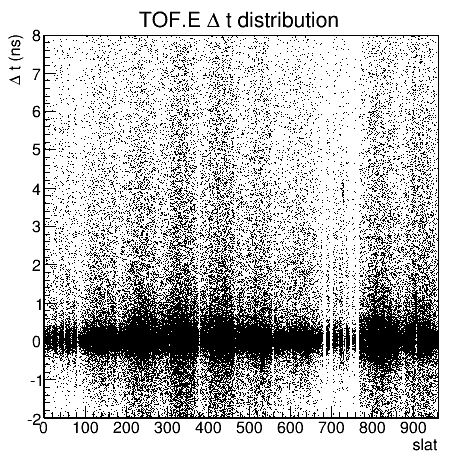
\includegraphics[width=0.5\textwidth]{evtQA/ttofedist.JPG}
    \rule{35em}{0.5pt}
  \caption[Timing calibration in the TOF.E]{Timing calibration in the TOF.E, $\Delta$t vs TOF.E slat number}
  \label{fig:tofedist}
\end{figure}
\begin{figure}[htbp]
  \centering
    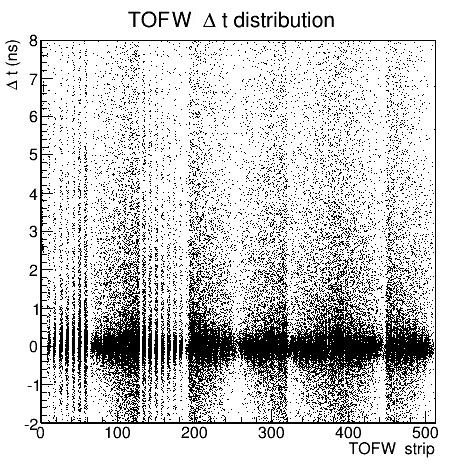
\includegraphics[width=0.5\textwidth]{evtQA/ttofwdist.JPG}
    \rule{35em}{0.5pt}
  \caption[Timing calibration in the TOF.W]{Timing calibration in the TOF.W, $\Delta$t vs TOF.W strip id}
  \label{fig:tofwdist}
\end{figure}

\pagebreak
\pagebreak
